\chapter{Objetivos}
\label{cap:capitulo2}

\begin{flushright}
\begin{minipage}[]{10cm}
\emph{Dame seis horas para talar un árbol y pasaré las primeras cuatro afilando el hacha}\\
\end{minipage}\\

Abraham Licoln\\
\end{flushright}

\vspace{1cm}

Una vez establecido el marco contextual de este proyecto, se procederá a
presentar una descripción del problema abordado, así como el proceso creativo e
intelectual que ha guiado el desarrollo del mismo, que incluirá los requisitos
del proyecto, la metodología empleada y el plan de trabajo detallado.

%Escribe aquí un párrafo explicando brevemente lo que vas a contar en este capítulo. En este capítulo lo ideal es explicar cuáles han sido los objetivos que te has fijado conseguir con tu trabajo, qué requisitos ha de respetar el resultado final, y cómo lo has llevado a cabo; esto es, cuál ha sido tu plan de trabajo.\\

\section{Descripción del problema}
\label{sec:descripcion}

Este proyecto surge como respuesta a la escasa investigación sobre los flujos de
datos en conjunto con ROS2, ofreciendo a su vez un entorno propicio para la
creación sencilla de distintas aplicaciones robóticas basadas en dichos flujos
de datos, que pueden replicar de manera versátil y sencilla, los comportamientos
reativos de los robots, eludiendo la complejidad inherente de este
\textit{middleware} robótico y dando lugar, por tanto, a un nuevo entorno de
programación más simple.

Además, tiene como objetivo secundario cerrar la brecha educativa entre la
enseñanza secundaria y universitaria, expuesta en la Sección
\ref{sec:educacion_robotica}, en la que queda explicado el salto que existe en
la educación en robótica entre la educación secundaria y la universitaria,
debido a la complejidad del código y de las plataformas de desarrollo
utilizadas.

%Cuenta aquí el objetivo u objetivos generales y, a continuación, concrétalos mediante objetivos específicos.

\section{Requisitos}
\label{sec:requisitos}

Para solucionar lso problemas descritos, este trabajo debe cumplir los
siguientes requisitos:

\begin{enumerate}
    \item{Se utilizará \textit{GNU/Linux}, con la distribución
        \textit{Ubuntu 22.04 LTS} como sistema operativo en todos los
        \textit{hardwares}.}
    \item{Desarrollar alguna forma de programación de flujos de datos con ROS2.}
    \item{El entorno de programación debe brindar la posibilidad de funcionar en
        conjunto con nodos de ROS2, permitiendo la comunicación con los mismos
        mediante \textit{topics}.}
    \item{Los \textit{softwares} utilizados deben ser compatibles para funcionar
        correctamente en conjunto.}
    \item{Las aplicaciones demostrativas desarrolladas deben ser fácilmente
        reproducibles y desplegables tanto en un entorno simulado como en un
        ambiente educativo real o de laboratorio.}
    \item{El desarrollo del \textit{software} debe ser lo suficientemente
        sencillo para poder ser llevado a cabo por alumnos preuniversitarios.}
    \item{El \textit{hardware} utilizado debe ser suficientemente económico para
        ser adquirido por organismos educativos.}
\end{enumerate}

Las competencias generales que se han cumplido, según la guía docente de la
asignatura consisten en:

\begin{enumerate}
    \item{\textit{CB2.} Que los estudiantes sepan aplicar sus conocimientos a su
        trabajo o vocación de una forma profesional y posean las competencias
        que suelen demostrarse por medio de la elaboración y defensa de
        argumentos y la resolución de problemas dentro de su área de estudio.}
        Esta competencia ha sido cumplida con la realización de la parte del
        software de este trabajo, en la que se han aplicado distintos
        conocimientos adquiridos durante el grado.
    \item{\textit{CB4.} Que los estudiantes puedan transmitir información,
        ideas, problemas y soluciones a un público tanto especializado como no
        especializado.}
        Esta competencia queda resuelta al detallar todo el complejo proceso
        consecuente a este trabajo de manera clara y comprensible en la memoria
        que esta siendo leída.
    \item{\textit{CB5.} Que los estudiantes hayan desarrollado aquellas
        habilidades de aprendizaje necesarias para emprender estudios
        posteriores con un alto grado de autonomía.}
        Esta competencia queda cumplida al haber adquirido los conocimientos
        suficientes para el desarrollo de este trabajo de manera completamente
        autónoma, a base de distintas pruebas y consultas en Internet.
\end{enumerate}

La competencia específica \textit{CE28} de la asignatura detalla lo
siguiente:
Desarrollo de las capacidades adecuadas para realizar un ejercicio original
individual (o excepcionalmente colectivo), presentarlo y defenderlo ante un
tribunal universitario, consistente en un proyecto en el ámbito de las
tecnologías específicas del campo de la Robótica de naturaleza profesional en el
que se sinteticen e integren las competencias adquiridas en las enseñanzas.
Esta última queda cumplida con la creación del presente trabajo, de la
consecuente memoria y documentación y de su posterior defensa ante un tribunal.

%Describe los requisitos que ha de cumplir tu trabajo.

\section{Metodología}
\label{sec:metodologia}

La metodología utilizada sigue pautas de invesigación sobre el estado del arte
previo al trabajo, y posteriormente sobre el \textit{software} utilizado,
siempre evaluando de antemano la compatibilidad con el \textit{hardware}
disponible, así como realizando pruebas pertinentes sobre su correcto
funcionamiento en los distintos entornos, incluyendo la simulación y el
laboratorio.

En relación con el desarrollo del \textit{software} demostrativo se sigió un
ciclo de desarrollo \textit{software} iterativo, que consiste en la
planificación del \textit{software}, el desarrollo del mismo, su consecuente
revisión mediante pruebas y su corrección, todo ello de manera periódica,
generando en cada una de las iteraciones un resultado ejecutable mejor que el
anterior, hasta conseguir al final una versión completamente funcional, como se
ve reflejado en el esquema de la Figura \ref{fig:desarrollo_iterativo}.
Este proceso de desarrollo puede verse alineado con los principios de mejora
continua del ciclo de desarrollo PDCA.

\begin{figure} [h!]
    \begin{center}
      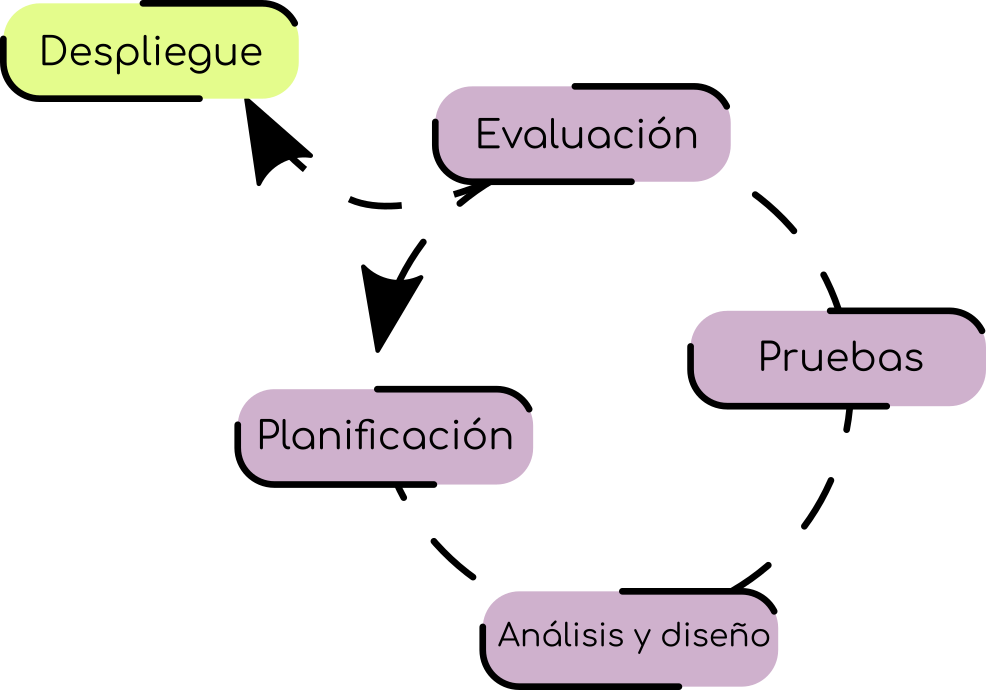
\includegraphics[width=12cm]{figs/desarrollo_iterativo}
    \end{center}
    \caption{Esquema del desarrollo software iterativo.}
    \label{fig:desarrollo_iterativo}
  \end{figure}\

Este desarrollo implicó pruebas periódicas en simulación con el fin de
identificar errores y perfeccionar los valores de los parámetros, para
posteriormente evaluar su funcionamiento en un entorno real, como el del
laboratorio.

%Qué paradigma de desarrollo software has seguido para alcanzar tus objetivos.

\section{Plan de trabajo}
\label{sec:plantrabajo}

El desarrollo del proyecto ha comprendido varias etapas, incluyendo la
investigación del \textit{software} a utilizar, la investigación del estado del
arte, la implementación de una arquitectura \textit{software} funcional en los
distintos entornos y el desarrollo del \textit{software} demostrativo o de
ejemplo, comprendiendo un periodo de tiempo superior a un año, comenzando en
Febrero de 2023 y finalizando en Mayo de 2024.

% [TODO] modificar la fecha final.

\begin{enumerate}
    \item{\textit{Investigación del software a utilizar.} Periodo de febrero a
        mayo de 2023 durante las prácticas de empresa, en las que estuve
        aprendiendo el funcionamiento de \textit{softwares} como Zenoh,
        Zenoh-Flow, Zenoh-bridge-DDS, CycloneDDS, y acerca de las
        telecomunicaciones entre robots, 35 horas semanales durante 4 meses.}
    \item{\textit{Investigación del estado del arte.} Periodo de junio a agosto
        de 2023, en el que se investigó acerca de los trabajos previos
        relacionados, y sobre la viabilidad y compatibilidad del proyecto.}
    \item{\textit{Implementación de una arquitectura software funcional en
        simulación.} Periodo de junio a agosto de 2023, en el que se consiguió
        un corecto funcionamiento del \textit{software} en simulación.}
    \item{\textit{Desarrollo de software demostrativo.} Periodo de agosto a
        noviembre de 2023 en el que se migró el \textit{software} desarrollado
        durante las prácticas a versiones posteriores.}
    \item{\textit{Implementación de una arquitectura software funcional en un
        entorno real.} Periodo de noviembre de 2023 a enero de 2024 en el que se
        consiguió un corecto funcionamiento del \textit{software} en el
        laboratorio.}
    \item{\textit{Pruebas del software desarrollado en el laboratorio.} Periodo
        de noviembre de 2023 a abril de 2024 en el que se realizaron las pruebas
        y cambios necesarios para un corecto funcionamiento del
        \textit{software} demostrativo en el entorno real del labratorio.}
\end{enumerate}

Durante los periodos de desarrollo de este proyecto fuera de las prácticas de
empresa, se dedcaban aproximadamente de 30 a 40 horas semanales entre las que se
incluyen reuniones con el tutor, que generalmente se llevaban a cabo
semanalemente aunque ocasionalmente cada dos semanas.
Este proceso continuo dió lugar a más de un año de esfuerzo.

El proceso de trabajo ha sido realizado mediante contribuciones a un repositorio
en GitHub\footnote{https://github.com/RoboticsURJC/tfg-unai}, así como su
posterior explicación y desarrollo en el apartado de la
Wiki\footnote{https://github.com/RoboticsURJC/tfg-unai/wiki} del mismo, haciendo
las veces de bitácora, donde quedan reflejados todos los contratiempos,
soluciones y pruebas realizados.

%Qué agenda has seguido. Si has ido manteniendo reuniones semanales, cumplimentando objetivos parciales, si has ido afinando poco a poco un producto final completo, etc.
